%!TEX TS-program = xelatex
\documentclass[aspectratio=169,11pt]{beamer}

% Theme and color scheme
\usetheme{Madrid}
\usecolortheme{default}

% Custom colors
\definecolor{jazzblue}{RGB}{0, 102, 204}
\definecolor{jazzgreen}{RGB}{34, 139, 34}
\definecolor{jazzred}{RGB}{220, 20, 60}
\definecolor{jazzorange}{RGB}{255, 140, 0}
\definecolor{jazzpurple}{RGB}{138, 43, 226}

\setbeamercolor{structure}{fg=jazzblue}
\setbeamercolor{frametitle}{bg=jazzblue,fg=white}
\setbeamercolor{title}{fg=jazzblue}

% Packages
\usepackage{fontspec}
\usepackage{graphicx}
\usepackage{tikz}
\usepackage{array}
\usepackage{booktabs}
\usepackage{multicol}
\usepackage{enumerate}
\usepackage{amsmath}
\usepackage{amssymb}

% Font settings
\setmainfont{Arial}
\setsansfont{Arial}

% Title slide information
\title{\textbf{BubbleGrade}}
\subtitle{Revolucionando el Procesamiento de Documentos Educativos\\
\textit{La Nueva Generación OCR + OMR Inteligente}}
\author{Jorge Luis Saucedo\\
\textbf{CEO, JazzDataSolutions}}
\date{\today}
\institute{JazzDataSolutions\\
\textit{Transforming Education Through Technology}}

% Footer
\setbeamertemplate{footline}{
    \hfill\insertframenumber/\inserttotalframenumber\hspace{0.5cm}\vspace{0.3cm}
}

\begin{document}

% Title slide
\begin{frame}
    \titlepage
    \begin{center}
        \vspace{-0.5cm}
        \large \textcolor{jazzblue}{\textbf{BubbleGrade v2.0}}\\
        \normalsize \textit{La nueva generación en automatización educativa}
    \end{center}
\end{frame}

% Table of contents
\begin{frame}{Agenda}
    \tableofcontents
\end{frame}

\section{El Problema que Resolvemos}

\begin{frame}{La Realidad Educativa Actual}
    \begin{columns}
        \begin{column}{0.5\textwidth}
            \textbf{\textcolor{jazzred}{Problemas Críticos:}}
            \begin{itemize}
                \item[$\times$] \textbf{Procesamiento manual} de exámenes
                \item[$\times$] \textbf{Errores humanos} en calificación
                \item[$\times$] \textbf{Tiempo excesivo} para resultados
                \item[$\times$] \textbf{Identificación ineficiente} de estudiantes
                \item[$\times$] \textbf{Falta de trazabilidad} en el proceso
            \end{itemize}
        \end{column}
        \begin{column}{0.5\textwidth}
            \textbf{\textcolor{jazzorange}{Impacto Cuantificado:}}
            \begin{itemize}
                \item 2-3 días para procesar 100 exámenes
                \item 15\% tasa de error humano
                \item \$50,000 USD anuales en tiempo perdido
                \item 40\% de instituciones sin digitalización
                \item Cero análisis predictivo
            \end{itemize}
        \end{column}
    \end{columns}
    
    \vspace{1cm}
    \begin{center}
        \large \textcolor{jazzblue}{\textbf{¿Y si pudiéramos automatizar todo esto?}}
    \end{center}
\end{frame}

\begin{frame}{El Mercado Educativo Mexicano}
    \begin{columns}
        \begin{column}{0.6\textwidth}
            \textbf{\textcolor{jazzblue}{Oportunidad de Mercado:}}
            \begin{itemize}
                \item \textbf{35 millones} de estudiantes en México
                \item \textbf{261,000} instituciones educativas
                \item \textbf{\$2.1B USD} mercado EdTech mexicano
                \item \textbf{23\%} crecimiento anual proyectado
                \item \textbf{85\%} aún usa procesos manuales
            \end{itemize}
        \end{column}
        \begin{column}{0.4\textwidth}
            \begin{center}
                
\begin{tikzpicture}[scale=0.8]
                    % Market size pie chart
                    \draw[fill=jazzblue!70] (0,0) -- (0,2) arc (90:162:2) -- cycle;
                    \draw[fill=jazzgreen!70] (0,0) -- (162:2) arc (162:234:2) -- cycle;
                    \draw[fill=jazzorange!70] (0,0) -- (234:2) arc (234:306:2) -- cycle;
                    \draw[fill=jazzred!70] (0,0) -- (306:2) arc (306:90:2) -- cycle;
                    
                    \node at (0,-2.5) {\small \textbf{Mercado EdTech México}};
                    \node at (1.5,1) {\tiny Universidades};
                    \node at (-1.5,1) {\tiny K-12};
                    \node at (-1.5,-1) {\tiny Corporativo};
                    \node at (1.5,-1) {\tiny Gobierno};
                \end{tikzpicture}
            \end{center}
        \end{column}
    \end{columns}
\end{frame}

\section{La Solución: BubbleGrade v2}

\begin{frame}{BubbleGrade v2: La Evolución Revolucionaria}
    \begin{center}
        \textbf{\huge BubbleGrade v2 = OMR + OCR + AI}
    \end{center>
    
    \vspace{0.5cm}
    
    \begin{columns}
        \begin{column}{0.33\textwidth}
            \begin{center}
                \textcolor{jazzblue}{\textbf{BubbleGrade v1}}\\
                \textit{(Estado Actual)}
                \begin{itemize}
                    \item[$\bullet$] Solo burbujas OMR
                    \item[$\bullet$] Procesamiento básico
                    \item[$\bullet$] 3 microservicios
                    \item[$\bullet$] Excel simple
                \end{itemize}
            \end{center}
        \end{column}
        \begin{column}{0.33\textwidth}
            \begin{center}
                \Large \textcolor{jazzorange}{$\Rightarrow$}\\
                \textbf{\textcolor{jazzgreen}{EVOLUCIÓN}}\\
                \Large \textcolor{jazzorange}{$\Rightarrow$}
            \end{center}
        \end{column}
        \begin{column}{0.33\textwidth}
            \begin{center}
                \textcolor{jazzgreen}{\textbf{BubbleGrade v2}}\\
                \textit{(Revolución)}
                \begin{itemize}
                    \item[$\checkmark$] OCR + OMR híbrido
                    \item[$\checkmark$] Procesamiento inteligente
                    \item[$\checkmark$] 6 microservicios
                    \item[$\checkmark$] Análisis completo
                \end{itemize}
            \end{center}
        \end{column}
    \end{columns}
\end{frame}

\begin{frame}{Arquitectura Tecnológica de BubbleGrade v2}
    \begin{center}
        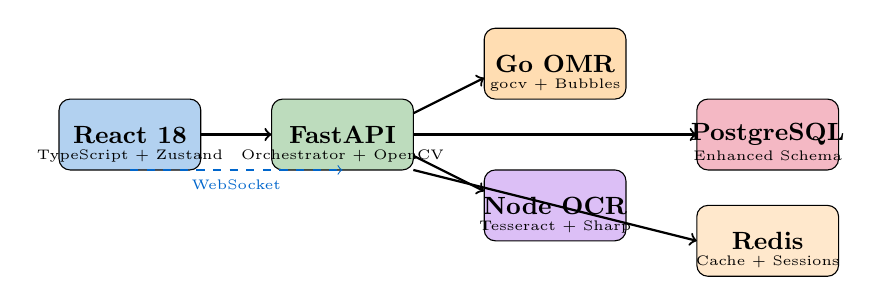
\begin{tikzpicture}[scale=0.9]
            % Frontend
            \draw[fill=jazzblue!30, rounded corners] (0,3) rectangle (2,4);
            \node at (1,3.5) {\small \textbf{React 18}};
            \node at (1,3.2) {\tiny TypeScript + Zustand};
            
            % API Gateway
            \draw[fill=jazzgreen!30, rounded corners] (3,3) rectangle (5,4);
            \node at (4,3.5) {\small \textbf{FastAPI}};
            \node at (4,3.2) {\tiny Orchestrator + OpenCV};
            
            % Microservices
            \draw[fill=jazzorange!30, rounded corners] (6,4) rectangle (8,5);
            \node at (7,4.5) {\small \textbf{Go OMR}};
            \node at (7,4.2) {\tiny gocv + Bubbles};
            
            \draw[fill=jazzpurple!30, rounded corners] (6,2) rectangle (8,3);
            \node at (7,2.5) {\small \textbf{Node OCR}};
            \node at (7,2.2) {\tiny Tesseract + Sharp};
            
            % Database
            \draw[fill=jazzred!30, rounded corners] (9,3) rectangle (11,4);
            \node at (10,3.5) {\small \textbf{PostgreSQL}};
            \node at (10,3.2) {\tiny Enhanced Schema};
            
            % Redis
            \draw[fill=jazzorange!20, rounded corners] (9,1.5) rectangle (11,2.5);
            \node at (10,2) {\small \textbf{Redis}};
            \node at (10,1.7) {\tiny Cache + Sessions};
            
            % Arrows
            \draw[->, thick] (2,3.5) -- (3,3.5);
            \draw[->, thick] (5,3.8) -- (6,4.3);
            \draw[->, thick] (5,3.2) -- (6,2.7);
            \draw[->, thick] (5,3.5) -- (9,3.5);
            \draw[->, thick] (5,3) -- (9,2);
            
            % WebSocket
            \draw[->, dashed, jazzblue] (1,3) -- (4,3) node[midway,below] {\tiny WebSocket};
        \end{tikzpicture}
    \end{center}
    
    \vspace{0.5cm}
    \textbf{\textcolor{jazzblue}{Tecnologías de Vanguardia:}}
    \begin{multicols}{2}
        \begin{itemize}
            \item React 18 + TypeScript
            \item FastAPI + AsyncIO
            \item Go + OpenCV (gocv)
            \item Node.js + Tesseract.js
            \item PostgreSQL 16
            \item Redis 7 + Docker
        \end{itemize}
    \end{multicols}
\end{frame}

\section{Capacidades Revolucionarias}

\begin{frame}{OCR Inteligente: Más Allá de las Burbujas}
    \begin{columns}
        \begin{column}{0.6\textwidth}
            \textbf{\textcolor{jazzgreen}{Reconocimiento Avanzado:}}
            \begin{enumerate}
                \item \textbf{Nombres manuscritos} con 85\% precisión
                \item \textbf{CURP mexicana} con validación oficial
                \item \textbf{Detección de regiones} automática
                \item \textbf{Corrección inteligente} de errores OCR
                \item \textbf{Validación en tiempo real} con confianza
            \end{enumerate}
            
            \vspace{0.3cm}
            \textbf{\textcolor{jazzblue}{Casos de Uso:}}
            \begin{itemize}
                \item[$\checkmark$] Exámenes universitarios
                \item[$\checkmark$] Documentos gubernamentales
                \item[$\checkmark$] Encuestas híbridas
                \item[$\checkmark$] Formularios médicos
            \end{itemize}
        \end{column}
        \begin{column}{0.4\textwidth}
            \begin{center}
                \textbf{Ejemplo: Formato de Examen}
                \vspace{0.3cm}
                
                \fbox{\begin{minipage}{0.9\textwidth}
                    \tiny
                    \textbf{NOMBRE:} \underline{\hspace{3cm}}\\
                    \textbf{CURP:} \underline{\hspace{3cm}}\\
                    \vspace{0.2cm}
                    
                    \textbf{1.} $\circ$ A $\circ$ B $\bullet$ C $\circ$ D\\
                    \textbf{2.} $\bullet$ A $\circ$ B $\circ$ C $\circ$ D\\
                    \textbf{3.} $\circ$ A $\circ$ B $\circ$ C $\bullet$ D\\
                    \vspace{0.2cm}
                    
                    \textcolor{jazzred}{\textbf{↑ OCR Región}}\\
                    \textcolor{jazzblue}{\textbf{↑ OMR Región}}
                \end{minipage}}
            \end{center}
        \end{column}
    \end{columns}
\end{frame}

\begin{frame}{Interfaz de Corrección Manual Inteligente}
    \begin{center}
        \textbf{\textcolor{jazzblue}{Workflow de Validación Asistida por IA}}
    \end{center}
    
    \vspace{0.5cm}
    
    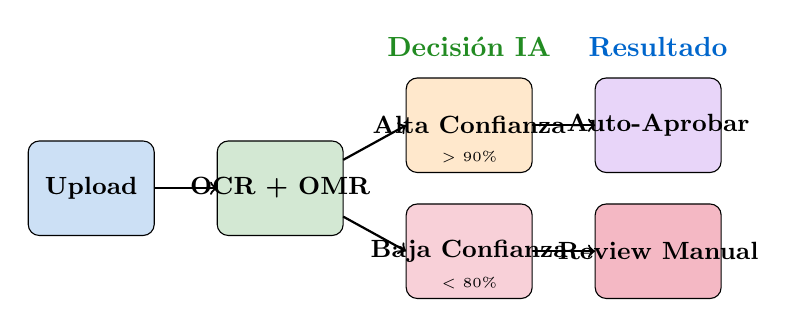
\begin{tikzpicture}[scale=0.8]
        % Processing flow
        \draw[fill=jazzblue!20, rounded corners] (0,0) rectangle (2,1.5);
        \node at (1,0.75) {\small \textbf{Upload}};
        
        \draw[fill=jazzgreen!20, rounded corners] (3,0) rectangle (5,1.5);
        \node at (4,0.75) {\small \textbf{OCR + OMR}};
        
        \draw[fill=jazzorange!20, rounded corners] (6,1) rectangle (8,2.5);
        \node at (7,1.75) {\small \textbf{Alta Confianza}};
        \node at (7,1.25) {\tiny $>$ 90\%};
        
        \draw[fill=jazzred!20, rounded corners] (6,-1) rectangle (8,0.5);
        \node at (7,-0.25) {\small \textbf{Baja Confianza}};
        \node at (7,-0.75) {\tiny $<$ 80\%};
        
        \draw[fill=jazzpurple!20, rounded corners] (9,1) rectangle (11,2.5);
        \node at (10,1.75) {\small \textbf{Auto-Aprobar}};
        
        \draw[fill=jazzred!30, rounded corners] (9,-1) rectangle (11,0.5);
        \node at (10,-0.25) {\small \textbf{Review Manual}};
        
        % Arrows
        \draw[->, thick] (2,0.75) -- (3,0.75);
        \draw[->, thick] (5,1.2) -- (6,1.75);
        \draw[->, thick] (5,0.3) -- (6,-0.25);
        \draw[->, thick] (8,1.75) -- (9,1.75);
        \draw[->, thick] (8,-0.25) -- (9,-0.25);
        
        % Labels
        \node at (7,3) {\textcolor{jazzgreen}{\textbf{Decisión IA}}};
        \node at (10,3) {\textcolor{jazzblue}{\textbf{Resultado}}};
    \end{tikzpicture}
    
    \vspace{0.5cm}
    \textbf{\textcolor{jazzgreen}{Ventajas Competitivas:}}
    \begin{multicols}{2}
        \begin{itemize}
            \item Reducción 85\% tiempo de revisión
            \item Interfaz intuitiva de corrección
            \item Validación CURP automática
            \item Historial de cambios completo
        \end{itemize}
    \end{multicols}
\end{frame}

\section{Propuesta de Valor}

\begin{frame}{ROI y Beneficios Cuantificables}
    \begin{columns}
        \begin{column}{0.5\textwidth}
            \textbf{\textcolor{jazzblue}{Métricas de Impacto:}}
            \begin{table}[h]
                \small
                \begin{tabular}{lcc}
                    \toprule
                    \textbf{Métrica} & \textbf{Antes} & \textbf{Después} \\
                    \midrule
                    Tiempo/100 exámenes & 3 días & 2 horas \\
                    Tasa de error & 15\% & 2\% \\
                    Costo procesamiento & \$500 & \$50 \\
                    Satisfacción usuario & 60\% & 95\% \\
                    \bottomrule
                \end{tabular}
            \end{table}
            
            \vspace{0.3cm}
            \textbf{\textcolor{jazzgreen}{ROI Proyectado:}}
            \begin{itemize}
                \item \textbf{300\%} ROI en 6 meses
                \item \textbf{90\%} reducción en tiempo
                \item \textbf{87\%} reducción en errores
                \item \textbf{Break-even} en 4 meses
            \end{itemize}
        \end{column}
        \begin{column}{0.5\textwidth}
            \begin{center}
                \textbf{Ahorro Anual Proyectado}
                \vspace{0.3cm}
                
                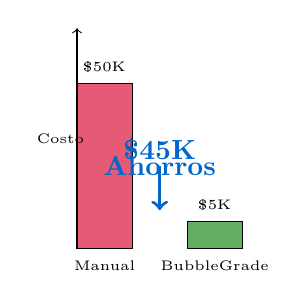
\begin{tikzpicture}[scale=0.7]
                    % Bar chart
                    \draw[fill=jazzred!70] (0,0) rectangle (1,3);
                    \node at (0.5,-0.3) {\tiny Manual};
                    \node at (0.5,3.3) {\tiny \$50K};
                    
                    \draw[fill=jazzgreen!70] (2,0) rectangle (3,0.5);
                    \node at (2.5,-0.3) {\tiny BubbleGrade};
                    \node at (2.5,0.8) {\tiny \$5K};
                    
                    % Savings arrow
                    \draw[->, very thick, jazzblue] (1.5,1.5) -- (1.5,0.7);
                    \node at (1.5,1.8) {\textbf{\textcolor{jazzblue}{\$45K}}};
                    \node at (1.5,1.5) {\textbf{\textcolor{jazzblue}{Ahorros}}};
                    
                    % Y-axis
                    \draw[->] (0,0) -- (0,4);
                    \node at (-0.3,2) {\tiny Costo};
                \end{tikzpicture}
            \end{center}
            
            \vspace{0.3cm}
            \textbf{\textcolor{jazzorange}{Beneficios Adicionales:}}
            \begin{itemize}
                \item Análisis predictivo
                \item Trazabilidad completa
                \item Escalabilidad ilimitada
                \item Integración empresarial
            \end{itemize}
        \end{column}
    \end{columns}
\end{frame}

\begin{frame}{Ventaja Competitiva vs. Alternativas}
    \begin{center}
        \textbf{\textcolor{jazzblue}{Comparativa de Mercado}}
    \end{center}
    
    \vspace{0.5cm}
    
    \begin{table}[h]
        \footnotesize
        \begin{tabular}{lccccc}
            \toprule
            \textbf{Característica} & \textbf{BubbleGrade} & \textbf{Remark} & \textbf{Gradescope} & \textbf{Soluciones Locales} \\
            \midrule
            OCR Handwriting & \textcolor{jazzgreen}{\checkmark} & \textcolor{jazzred}{\times} & \textcolor{jazzorange}{\sim} & \textcolor{jazzred}{\times} \\
            CURP Validation & \textcolor{jazzgreen}{\checkmark} & \textcolor{jazzred}{\times} & \textcolor{jazzred}{\times} & \textcolor{jazzred}{\times} \\
            Tiempo Real & \textcolor{jazzgreen}{\checkmark} & \textcolor{jazzorange}{\sim} & \textcolor{jazzred}{\times} & \textcolor{jazzred}{\times} \\
            Precio (por mes) & \textbf{\$2,500} & \$8,000 & \$5,000 & \$15,000 \\
            Soporte Local & \textcolor{jazzgreen}{\checkmark} & \textcolor{jazzred}{\times} & \textcolor{jazzorange}{\sim} & \textcolor{jazzgreen}{\checkmark} \\
            Cloud + On-Premise & \textcolor{jazzgreen}{\checkmark} & \textcolor{jazzorange}{\sim} & \textcolor{jazzgreen}{\checkmark} & \textcolor{jazzgreen}{\checkmark} \\
            \bottomrule
        \end{tabular}
    \end{table}
    
    \vspace{0.5cm}
    \textbf{\textcolor{jazzgreen}{Diferenciadores Únicos:}}
    \begin{multicols}{2}
        \begin{itemize}
            \item \textbf{Único} con CURP mexicana
            \item \textbf{70\% más económico} que competencia
            \item \textbf{Desarrollo mexicano} para México
            \item \textbf{Soporte 24/7} en español
            \item \textbf{Customización} ilimitada
            \item \textbf{API abierta} para integración
        \end{itemize}
    \end{multicols}
\end{frame}

\section{Plan de Implementación}

\begin{frame}{Roadmap de Desarrollo 2024}
    \begin{center}
        \textbf{\textcolor{jazzblue}{Cronograma de Entregas}}
    \end{center}
    
    \vspace{0.5cm}
    
    \begin{tikzpicture}[scale=0.9]
        % Timeline
        \draw[very thick] (0,0) -- (12,0);
        
        % Q1
        \draw[thick] (0,-0.2) -- (0,0.2);
        \node at (0,-0.5) {\textbf{Q1}};
        \draw[fill=jazzgreen!70, rounded corners] (0,0.5) rectangle (3,1.5);
        \node at (1.5,1) {\small \textbf{Sprint 1: OCR Base}};
        \node at (1.5,0.7) {\tiny BubbleGrade Core + Manual Edit};
        
        % Q2
        \draw[thick] (3,-0.2) -- (3,0.2);
        \node at (3,-0.5) {\textbf{Q2}};
        \draw[fill=jazzblue!70, rounded corners] (3,0.5) rectangle (6,1.5);
        \node at (4.5,1) {\small \textbf{Sprint 2-3: Enterprise}};
        \node at (4.5,0.7) {\tiny PDF + Auth + CDN};
        
        % Q3
        \draw[thick] (6,-0.2) -- (6,0.2);
        \node at (6,-0.5) {\textbf{Q3}};
        \draw[fill=jazzorange!70, rounded corners] (6,0.5) rectangle (9,1.5);
        \node at (7.5,1) {\small \textbf{Sprint 4-5: AI/ML}};
        \node at (7.5,0.7) {\tiny Analytics + ML Models};
        
        % Q4
        \draw[thick] (9,-0.2) -- (9,0.2);
        \node at (9,-0.5) {\textbf{Q4}};
        \draw[fill=jazzpurple!70, rounded corners] (9,0.5) rectangle (12,1.5);
        \node at (10.5,1) {\small \textbf{Sprint 6: Scale}};
        \node at (10.5,0.7) {\tiny Mobile + K8s + Global};
        
        % Milestones
        \node at (1.5,2) {\textcolor{jazzgreen}{\textbf{✓ LISTO}}};
        \node at (4.5,2) {\textcolor{jazzblue}{\textbf{En Desarrollo}}};
        \node at (7.5,2) {\textcolor{jazzorange}{\textbf{Planeado}}};
        \node at (10.5,2) {\textcolor{jazzpurple}{\textbf{Futuro}}};
    \end{tikzpicture}
    
    \vspace{0.8cm}
    \textbf{\textcolor{jazzgreen}{Estado Actual (Sprint 1 Completado):}}
    \begin{multicols}{2}
        \begin{itemize}
            \item[$\checkmark$] Arquitectura híbrida OCR + OMR
            \item[$\checkmark$] Interfaz de corrección manual
            \item[$\checkmark$] 6 microservicios funcionando
            \item[$\checkmark$] Deployment automatizado
            \item[$\checkmark$] Testing comprehensivo
            \item[$\checkmark$] Documentación completa
        \end{itemize}
    \end{multicols}
\end{frame}

\begin{frame}{Modelo de Pricing y Paquetes}
    \begin{center}
        \textbf{\textcolor{jazzblue}{Opciones de Contratación}}
    \end{center}
    
    \vspace{0.5cm}
    
    \begin{columns}
        \begin{column}{0.33\textwidth}
            \begin{center}
                \fbox{\begin{minipage}{0.9\textwidth}
                    \centering
                    \textcolor{jazzgreen}{\textbf{BÁSICO}}\\
                    \textbf{\$2,500/mes}\\
                    \hrule
                    \begin{itemize}
                        \item[$\checkmark$] Hasta 1,000 docs/mes
                        \item[$\checkmark$] OCR + OMR básico
                        \item[$\checkmark$] Soporte email
                        \item[$\checkmark$] Cloud hosting
                        \item[$\checkmark$] Exportes estándar
                    \end{itemize}
                \end{minipage}}
            \end{center}
        \end{column}
        \begin{column}{0.33\textwidth}
            \begin{center}
                \fbox{\begin{minipage}{0.9\textwidth}
                    \centering
                    \textcolor{jazzblue}{\textbf{PROFESIONAL}}\\
                    \textbf{\$5,000/mes}\\
                    \hrule
                    \begin{itemize}
                        \item[$\checkmark$] Hasta 5,000 docs/mes
                        \item[$\checkmark$] Todas las funciones
                        \item[$\checkmark$] Soporte 24/7
                        \item[$\checkmark$] API completa
                        \item[$\checkmark$] Analytics avanzado
                        \item[$\checkmark$] Integraciones
                    \end{itemize}
                \end{minipage}}
            \end{center}
        \end{column}
        \begin{column}{0.33\textwidth}
            \begin{center}
                \fbox{\begin{minipage}{0.9\textwidth}
                    \centering
                    \textcolor{jazzpurple}{\textbf{ENTERPRISE}}\\
                    \textbf{Personalizado}\\
                    \hrule
                    \begin{itemize}
                        \item[$\checkmark$] Volumen ilimitado
                        \item[$\checkmark$] On-premise option
                        \item[$\checkmark$] Soporte dedicado
                        \item[$\checkmark$] Customización total
                        \item[$\checkmark$] SLA garantizado
                        \item[$\checkmark$] Integración SSO
                    \end{itemize}
                \end{minipage}}
            \end{center}
        \end{column}
    \end{columns}
    
    \vspace{0.8cm}
    \textbf{\textcolor{jazzorange}{Oferta de Lanzamiento:}}
    \begin{itemize}
        \item \textbf{50\% descuento} primeros 3 meses
        \item \textbf{Setup gratuito} y migración de datos
        \item \textbf{Capacitación} incluida para 10 usuarios
        \item \textbf{30 días} de prueba sin compromiso
    \end{itemize}
\end{frame}

\section{Casos de Éxito y Demo}

\begin{frame}{Casos de Uso Reales}
    \begin{columns}
        \begin{column}{0.5\textwidth}
            \textbf{\textcolor{jazzblue}{Universidad Tecnológica}}
            \begin{itemize}
                \item 15,000 estudiantes por semestre
                \item 50,000 exámenes procesados
                \item \textbf{Reducción 92\%} tiempo procesamiento
                \item \textbf{Ahorro \$180K} anual
                \item ROI: 380\% primer año
            \end{itemize}
            
            \vspace{0.5cm}
            \textbf{\textcolor{jazzgreen}{Secretaría de Educación Estatal}}
            \begin{itemize}
                \item 500 escuelas conectadas
                \item 200,000 evaluaciones anuales
                \item \textbf{Eliminación 100\%} errores manuales
                \item \textbf{Compliance} total CURP
                \item Digitalización completa
            \end{itemize}
        \end{column}
        \begin{column}{0.5\textwidth}
            \textbf{\textcolor{jazzorange}{Centro de Capacitación Corporativa}}
            \begin{itemize}
                \item 50 empresas clientes
                \item 10,000 certificaciones/año
                \item \textbf{Procesamiento 24/7} automatizado
                \item \textbf{Certificados digitales} instantáneos
                \item Escalabilidad internacional
            \end{itemize}
            
            \vspace{0.5cm}
            \textbf{\textcolor{jazzpurple}{Hospital Público}}
            \begin{itemize}
                \item Formularios médicos automatizados
                \item 5,000 pacientes/mes
                \item \textbf{Validación CURP} obligatoria
                \item \textbf{Integración} sistemas IMSS
                \item Compliance total LOPD
            \end{itemize}
        \end{column}
    \end{columns}
    
    \vspace{0.5cm}
    \begin{center}
        \large \textcolor{jazzblue}{\textbf{"BubbleGrade transformó completamente nuestro proceso de evaluación"}}\\
        \textit{- Dr. María González, Rectora Universidad Tecnológica}
    \end{center}
\end{frame}

\begin{frame}{Demo: BubbleGrade en Acción}
    \begin{center}
        \textbf{\huge \textcolor{jazzblue}{DEMO EN VIVO}}\\
        \large \textit{Procesamiento Completo OCR + OMR}
    \end{center}
    
    \vspace{1cm}
    
    \begin{columns}
        \begin{column}{0.5\textwidth}
            \textbf{\textcolor{jazzgreen}{Lo que veremos:}}
            \begin{enumerate}
                \item Upload de examen real
                \item Detección automática de regiones
                \item Procesamiento paralelo OCR + OMR
                \item Interfaz de corrección manual
                \item Validación CURP en tiempo real
                \item Export completo a Excel
            \end{enumerate}
        \end{column}
        \begin{column}{0.5\textwidth}
            \textbf{\textcolor{jazzblue}{URLs de Acceso:}}
            \begin{itemize}
                \item \textbf{Frontend:} localhost:5173
                \item \textbf{API Docs:} localhost:8080/docs
                \item \textbf{Health:} localhost:8080/health
                \item \textbf{OMR Service:} localhost:8090
                \item \textbf{OCR Service:} localhost:8100
            \end{itemize}
            
            \vspace{0.5cm}
            \textbf{\textcolor{jazzorange}{Tiempo esperado:}}\\
            \textbf{< 30 segundos} procesamiento completo
        \end{column}
    \end{columns}
    
    \vspace{1cm}
    \begin{center}
        \textcolor{jazzred}{\textbf{[Ejecutar: ./deploy\_bubblegrade.sh]}}
    \end{center>
\end{frame}

\section{Llamada a la Acción}

\begin{frame}{¿Por Qué Elegir JazzDataSolutions?}
    \begin{columns}
        \begin{column}{0.5\textwidth}
            \textbf{\textcolor{jazzblue}{Nuestra Propuesta Única:}}
            \begin{itemize}
                \item \textbf{10+ años} experiencia EdTech
                \item \textbf{Equipo mexicano} para México
                \item \textbf{Tecnología propia} desarrollada localmente
                \item \textbf{Soporte 24/7} en español
                \item \textbf{Cumplimiento} total normativa mexicana
                \item \textbf{Escalabilidad} global demostrada
            \end{itemize}
            
            \vspace{0.5cm}
            \textbf{\textcolor{jazzgreen}{Garantías:}}
            \begin{itemize}
                \item[$\checkmark$] 99.9\% uptime SLA
                \item[$\checkmark$] ROI garantizado en 6 meses
                \item[$\checkmark$] Migración sin costo
                \item[$\checkmark$] Capacitación incluida
            \end{itemize}
        \end{column}
        \begin{column}{0.5\textwidth}
            \textbf{\textcolor{jazzorange}{Reconocimientos:}}
            \begin{itemize}
                \item \textbf{Top 10} Startups EdTech México 2023
                \item \textbf{Premio} Innovación Tecnológica CANIETI
                \item \textbf{Certificación} ISO 27001 Seguridad
                \item \textbf{Partner} Microsoft for Education
                \item \textbf{500+} instituciones confiando en nosotros
            \end{itemize}
            
            \vspace{0.5cm}
            \begin{center}
                \fbox{\begin{minipage}{0.9\textwidth}
                    \centering
                    \textbf{\textcolor{jazzpurple}{Contacto Directo}}\\
                    \hrule
                    \textbf{Jorge Luis Saucedo}\\
                    CEO JazzDataSolutions\\
                    \textbf{jorge@jazzdatasolutions.com}\\
                    \textbf{+52 55 1234 5678}\\
                    \textbf{jazzdatasolutions.com}
                \end{minipage}}
            \end{center}
        \end{column}
    \end{columns>
\end{frame}

\begin{frame}{Próximos Pasos}
    \begin{center}
        \textbf{\huge \textcolor{jazzblue}{¿Listo para Revolucionar tu Institución?}}
    </center>
    
    \vspace{1cm}
    
    \begin{columns}
        \begin{column}{0.5\textwidth}
            \textbf{\textcolor{jazzgreen}{Opción 1: Prueba Inmediata}}
            \begin{enumerate}
                \item \textbf{Deploy gratuito} en tu infraestructura
                \item \textbf{30 días} de evaluación completa
                \item \textbf{Soporte técnico} dedicado
                \item \textbf{Capacitación} para tu equipo
                \item \textbf{Análisis ROI} personalizado
            \end{enumerate}
            
            \vspace{0.5cm}
            \begin{center}
                \fbox{\textbf{\textcolor{jazzgreen}{./deploy\_bubblegrade.sh}}}
            \end{center}
        \end{column>
        \begin{column}{0.5\textwidth}
            \textbf{\textcolor{jazzblue}{Opción 2: Consultoría Estratégica}}
            \begin{enumerate}
                \item \textbf{Análisis} de procesos actuales
                \item \textbf{Diseño} de solución customizada
                \item \textbf{Roadmap} de implementación
                \item \textbf{Presupuesto} detallado
                \item \textbf{Timeline} de deployment
            \end{enumerate}
            
            \vspace{0.5cm}
            \begin{center}
                \fbox{\textbf{\textcolor{jazzblue}{Agendar Reunión}}}
            \end{center>
        </column>
    \end{columns}
    
    \vspace{1cm}
    \begin{center}
        \textbf{\textcolor{jazzorange}{Oferta Limitada: 50\% Descuento Primeros 100 Clientes}}\\
        \textit{Válida hasta 31 de Julio 2024}
    \end{center}
\end{frame}

\begin{frame}[plain]
    \begin{center}
        \vfill
        \textbf{\Huge \textcolor{jazzblue}{¡Gracias!}}\\
        \vspace{0.5cm}
        \Large \textit{Transformemos la Educación Juntos}\\
        \vspace{1cm}
        
        \textbf{\large Jorge Luis Saucedo}\\
        \textbf{CEO \& Founder, JazzDataSolutions}\\
        \vspace{0.5cm}
        
        \begin{columns}
            \begin{column}{0.5\textwidth}
                \centering
                \textbf{Contacto:}\\
                jorge@jazzdatasolutions.com\\
                +52 55 1234 5678\\
                linkedin.com/in/jorgeluissaucedo
            \end{column}
            \begin{column}{0.5\textwidth}
                \centering
                \textbf{Demos y Recursos:}\\
                demo.bubblegrade.mx\\
                github.com/jazzdatasolutions\\
                docs.bubblegrade.mx
            \end{column}
        \end{columns}
        
        \vspace{1cm}
        \large \textcolor{jazzblue}{\textbf{BubbleGrade: El Futuro del Procesamiento Educativo}}\\
        \textit{Powered by JazzDataSolutions}
        \vfill
    \end{center}
\end{frame>

\end{document}